\section{Complex Numbers} \label{sec 8.d}

For the purposes of algebra, the field of real numbers is \emph{not sufficient}, for there are polynomials of \emph{nonzero degree} with \emph{real coefficients} that \textbf{have no zeros} in the field of real numbers (for example, \(x^2 + 1\)).
It is often desirable to have a field in which any polynomial of nonzero degree \emph{with coefficients from that field} has a \emph{zero in that field}.
It is possible to ``enlarge'' the field of real numbers to obtain such a field.

\begin{note}
\RED{Warning}: This section in fact uses some concepts defined later in \SEC{8.e}.
E.g. the definition of ``zeroes'' (see \RMK{e.2}), and the definition of the polynomial.
\end{note}

\begin{appendix definition} \label{def d.1}
A \textbf{complex number} is an expression of the form \(z = a + b \iu\), where \(a\) and \(b\) are \emph{real} numbers called the \textbf{real part} and the \textbf{imaginary part} of \(z\), respectively.
The \textbf{sum} and \textbf{product} of two complex numbers \(z = a + b \iu\) and \(w = c + d \iu\) (where \(a, b, c\), and \(d\) are real numbers) are defined, respectively, as follows:
\[
    z + w = (a + b\iu) + (c + d\iu) = (a + c) + (b + d) \iu
\]
and
\[
    zw = (a + b\iu)(c + d\iu) = (ac\ \RED{-}\ bd) + (bc + ad)\iu.
\]
\end{appendix definition}

\begin{note}
注意,這是複數的定義,而從這個定義出發,在後面的 \ \RMK{d.2} 我們可以得到\ \(\iu^2 = -1\)。
所以(至少在這本書裡) \(\iu^2 = -1\) 並不是定義出來的。
\end{note}

\begin{example} \label{example d.1}
The sum and product of \(z = 3 - 5\iu\) and \(w = 9 + 7\iu\) are, respectively,
\[
    z + w = (3 - 5\iu) + (9 + 7\iu) = (3 + 9) + [(-5) + 7]\iu = 12 + 2\iu
\]
and
\[
    zw = (3 - 5\iu)(9 + 7\iu) = [3 \cdot 9 - (-5) \cdot 7] + [(-5) \cdot 9 + 3 \cdot 7]\iu = 62 - 24\iu.
\]
\end{example}

\begin{remark} \label{remark d.1}
Any \emph{real} number \(c\) may be \emph{regarded as a complex number} by identifying \(c\) with the complex number \(c + 0\iu\),
that is, \emph{treating them as identical}.

Observe that this correspondence \emph{preserves sums and products} (of real numbers); that is,
\begin{align*}
    c + d & = (c + 0\iu) + (d + 0\iu) & \text{treating real as complex} \\
        & = (c + d) + (0 + 0)\iu & \text{by \DEF{d.1}} \\
        & = (c + d) + 0\iu & \text{by (F 3) of real number} \\
        & = c + d & \text{treating complex (whose imaginary part is zero) as real}
\end{align*}
and
\begin{align*}
    c \cdot d & = (c + 0\iu) \cdot (d + 0\iu) & \text{treating real as complex} \\
        & = (c \cdot d - 0 \cdot 0) + (0 \cdot d + c \cdot 0)\iu & \text{by \DEF{d.1}} \\
        & = (c \cdot d) + 0\iu & \text{by the field algebra of real number} \\
        & = c \cdot d & \text{treating complex (whose imaginary part is zero) as real}
\end{align*}
\end{remark}

\begin{remark} \label{remark d.2}
Any complex number of the form \(b \iu = 0 + b \iu\), where \(b\) is a \emph{nonzero} real number, is called \textbf{imaginary}.
The product of two imaginary numbers is real since
\begin{align*}
    (b\iu)(d\iu) & = (0 + b\iu)(0 + d\iu) \\
        & = (0 \cdot 0 - bd) + (b \cdot 0 + 0 \cdot d)\iu & \text{by \DEF{5.1}} \\
        & = (-bd) + 0\iu & \text{by the field algebra of real number} \\
        & = (-bd) & \text{treating complex (whose imaginary part is zero) as real}
\end{align*}

\textbf{In particular}, for \(\iu = 0 + 1\iu\), we have \(\iu \cdot \iu = (0 + 1\iu)(0 + 1\iu) = (-1 \cdot 1) = -1\).

The derived fact that \(\iu^2 = \iu \cdot \iu = -1\) provides an easy way to \emph{remember the definition} of multiplication of complex numbers:
simply multiply two complex numbers \textbf{as you would any two algebraic expressions}, and \textbf{replace \(\iu^2\) by \(-1\)}.

The next example illustrates this technique.
\end{remark}

\begin{example} \label{example d.2}
The product of \(-5 + 2\iu\) and \(1 - 3\iu\) is
\begin{align*}
    (-5 + 2\iu)(1 - 3\iu) & = -5(1 - 3\iu) + 2\iu(1 - 3\iu) & \text{by ``normal'' algebra, not by definition} \\
        & = -5 + 15\iu + 2\iu - 6\iu^2 & \text{just by ``normal'' distributive law} \\
        & = -5 + 15\iu + 2\iu - 6(-1) & \text{by replacing \(\iu^2\) by \(-1\)} \\
        & = 1 + 17\iu.
\end{align*}
\end{example}

\begin{remark} \label{remark d.3}
The \emph{real} number \(0\), when being regarded as a complex number, \emph{is} an \emph{additive identity} element for the complex numbers since
\begin{align*}
    (a + b\iu) + \RED{0} & = (a + b\iu) + (\RED{0} + 0\iu) & \text{treating real as complex} \\
        & = (a + 0) + (b + 0)\iu & \text{by \DEF{d.1}} \\
        & = a + b\iu. & \text{by the field algebra of real number}
\end{align*}

Likewise the \emph{real} number \(1\), regarded as a complex number, is a \emph{multiplicative identity} element for the set of complex numbers since
\begin{align*}
    (a + b\iu) \cdot \RED{1} & = (a + b\iu) \cdot (\RED{1} + 0\iu) & \text{treating real as complex} \\
        & = (a \cdot 1 - b \cdot 0) + (b \cdot 1 + a \cdot 0)\iu & \text{by \DEF{d.1}} \\
        & = a + b\iu. & \text{by the field algebra of real number}
\end{align*}

Every complex number \(a + b\iu\) has an additive inverse, namely \((-a) + (-b)\iu\).
But also each complex number \emph{except} \(0\) has a \emph{multiplicative inverse}; see the next theorem.
\end{remark}

\begin{appendix theorem} \label{thm d.1}
The set of complex numbers with the operations of addition and multiplication in \DEF{d.1} is a field.
\end{appendix theorem}

\begin{proof}
The addition and multiplication in \DEF{d.1} is of course well defined, so we only need to check (F 1) to (F 5) in \DEF{c.1}.

\begin{enumerate}
\item[(F 1)] Given any two complex numbers \(a + b \iu, c + d \iu\) where \(a, b, c, d \in \SET{R}\), we have
\begin{align*}
    (a + b\iu) + (c + d\iu) & = (a + c) + (b + d)\iu & \text{by \DEF{d.1}} \\
        & = (c + a) + (d + b)\iu & \text{by (F 1) of real numbers} \\
        & = (c + d\iu) + (a + b\iu) & \text{by \DEF{d.1} again}
\end{align*}
and
\begin{align*}
   (a + b\iu)(c + d\iu) & = (ac - bd) + (bc + ad)\iu & \text{by \DEF{d.1}} \\
        & = (ca - db) + (da + cb)\iu & \text{by applying (F 1) of real numbers many times} \\
        & = (c + d\iu)(a + b\iu) & \text{by \DEF{d.1} again}
\end{align*}

\item[(F 2)] Given any three complex numbers \(a + b \iu, c + d \iu, e + f \iu\) where \(a, b, c, d, e, f \in \SET{R}\), we have
\begin{align*}
    [(a + b\iu) + (c + d\iu)] + (e + f\iu) & = [(a + c) + (b + d)\iu] + (e + f\iu) & \text{by \DEF{d.1}} \\
        & = [(a + c) + e] + [(b + d) + f]\iu & \text{by \DEF{d.1} again} \\
        & = [a + (c + e)] + [b + (d + f)]\iu & \text{by (F 2) of real numbers} \\
        & = (a + b\iu) + [(c + e) + (d + f)\iu] & \text{by \DEF{d.1}} \\
        & = (a + b\iu) + [(c + d\iu) + (e + f\iu)]. & \text{by \DEF{d.1} again}
\end{align*}
For associativity of complex number, first,
\begin{align*}
    & [(a + b\iu)(c + d\iu)](e + f \iu) \\
    & = [(ac - bd) + (bc + ad)\iu] (e + f\iu) \\
    & \quad \quad \text{(by \DEF{d.1})} \\
    & = ((ac - bd)e - (bc + ad)f) + ((bc + ad)e + (ac - bd)f)\iu \\
    & \quad \quad \text{(by \DEF{d.1} again)} \\
    & = (ace - bde - bcf - adf) + (bce + ade + acf - bdf) \iu \\
    & \quad \quad \text{(just expanding by real number's algebra)} \\
    & = (ace - adf - bcf - bde) + (acf + ade + bce - bdf) \iu \quad \MAROON{(2.1)} \\
    & \quad \quad \text{(just rearranging according to lexical order)}
\end{align*}
and
\begin{align*}
    & (a + b \iu)[(c + d\iu)(e + f\iu)) \\
    & = (a + b\iu)[(ce - df) + (de + cf)\iu] \\
    & \quad \quad \text{(by \DEF{d.1})} \\
    & = (a(ce - df) - b(de + cf)) + (b(ce - df) + a(de + cf)) \iu \\
    & \quad \quad \text{(by \DEF{d.1} again)} \\
    & = (ace - adf - bde - bcf) + (bce - bdf + ade + acf)\iu \\
    & \quad \quad \text{(just expanding by real number's algebra)} \\
    & = (ace - adf - bcf - bde) + (acf + ade + bce - bdf)\iu \\
    & \quad \quad \text{(just rearranging according to lexical order)} \\
    & = \MAROON{(2.1)}
\end{align*}
Hence \([(a + b\iu)(c + d\iu)](e + f \iu) = (a + b \iu)[(c + d\iu)(e + f\iu)]\).

\item[(F 3)] This is shown in \RMK{d.3}.

\item[(F 4)] The additive inverse is shown in \RMK{d.3}.
Suppose \(a + b\iu \ne 0\) where \(a, b \in \SET{R}\).
Then we claim that
\[
    (a + b\iu)^{-1} = \left( \frac{a}{a^2 + b^2} \right) - \left( \frac{b}{a^2 + b^2} \right)\iu,
\]
since
\begin{align*}
    & (a + b\iu) \left[ \left( \frac{a}{a^2 + b^2} \right) - \left( \frac{b}{a^2 + b^2} \right)\iu \right] \\
    & = \left[ a \cdot \frac{a}{a^2 + b^2} - b \left( - \frac{b}{a^2 + b^2} \right) \right] + \left[ b \cdot \frac{a}{a^2 + b^2} + a \left( - \frac{b}{a^2 + b^2} \right) \right] \iu \\
    & \quad \quad \text{(by \DEF{d.1})} \\
    & = \frac{a^2 + b^2}{a^2 + b^2} + \frac{ab - ab}{a^2 + b^2} \iu \\
    & \quad \quad \text{(just using real number algebra)} \\
    & = 1 + 0 \iu = 1.
\end{align*}

\item[(F 5)] Given any three complex numbers \(a + b \iu, c + d \iu, e + f \iu\) where \(a, b, c, d \in \SET{R}\), we have
\begin{align*}
    & (a + b\iu)[(c + d\iu) + (e + f\iu)] \\
    & = (a + b\iu)[(c + e) + (d + f)\iu] & \text{by \DEF{5.1}} \\
    & = [a(c + e) - b(d + f)] + [b(c + e) + a(d + f)] \iu & \text{by \DEF{5.1} again} \\
    & = (ac + ae - bd - bf) + (bc + be + ad + af) \iu & \text{using real number algebra} \\
    & = (ac + ae - bd - bf) + (ad + af + bc + be) \iu \quad \MAROON{(5.1)} & \text{rearranging by lexical order} \\
\end{align*}
and
\begin{align*}
    & (a + b\iu)(c + d\iu) + (a + b\iu)(e + f\iu) \\
    & = [(ac - bd) + (bc + ad)\iu] + [(ae - bf) + (be + af)\iu] & \text{by \DEF{5.1}} \\
    & = [(ac - bd) + (ae - bf)] + [(bc + ad) + (be + af)] \iu & \text{by \DEF{5.1} again} \\
    & = (ac + ae - bd - bf) + (ad + af + bc + be) \iu & \text{rearranging by lexical order} \\
    & = \MAROON{(5.1)}
\end{align*}
So \((a + b\iu)[(c + d\iu) + (e + f\iu)] = (a + b\iu)(c + d\iu) + (a + b\iu)(e + f\iu)\).
\end{enumerate}
\end{proof}

\begin{appendix definition} \label{def d.2}
The \textbf{(complex) conjugate} of a complex number \(a + b\iu\) is the complex number \(a - b\iu\).
We denote the conjugate of the complex number \(z\) by \(\conjugatet{z}\).
\end{appendix definition}

\begin{example}
The conjugates of \(-3 + 2\iu\), \(4 - 7\iu\), and \(6\) are, respectively,
\(\conjugatet{-3 + 2\iu} = -3 - 2\iu\), \(\conjugatet{4 - 7\iu} = 4 + 7\iu\), and \(\conjugatet{6} = \conjugatet{6 + 0\iu} = \conjugatet{6 - 0\iu} = 6\).
\end{example}

The next theorem contains some important properties of the conjugate of a complex number.

\begin{appendix theorem} \label{thm d.2}
Let \(z\) and \(w\) be complex numbers.
Then the following statements are true.

\begin{enumerate}
\item \(\conjugatet{\conjugatet{z}} = z\).
\item \(\conjugatet{z + w} = \conjugatet{z} + \conjugatet{w}\).
\item \(\conjugatet{zw} = \conjugatet{z} \cdot \conjugatet{w}\).
\item \(\conjugatet{\left( \cfrac{z}{w} \right)} = \cfrac{\conjugatet{z}}{\conjugatet{w}}\) if \(w \ne 0\).
\item \(z\) is a real number if and only if \(\conjugatet{z} = z\).
\end{enumerate}
\end{appendix theorem}

\begin{proof} \ 

\begin{enumerate}
\item Let \(z = a + b\iu\), then \(\conjugatet{\conjugatet{z}} = \conjugatet{\conjugatet{a + b \iu}} = \conjugatet{a - b\iu} = a + b\iu = z\) where each step is derived by \DEF{d.2}.

\item Let \(z = a + b\iu\) and \(w = c + d\iu\), where \(a, b, c, d \in \SET{R}\).
Then
\begin{align*}
    \conjugatet{z + w} & = \conjugatet{(a + b\iu) + (c + d\iu)} = \conjugatet{(a + c) + (b + d)\iu} & \text{by \DEF{d.1}} \\
        & = (a + c) - (b + d)\iu & \text{by \DEF{d.2}} \\
        & = (a - b\iu) + (c - d\iu) & \text{by \DEF{d.1}} \\
        & = \conjugatet{a + b\iu} + \conjugatet{c + d\iu} & \text{by \DEF{d.2}} \\
        & = \conjugatet{z} + \conjugatet{w}.
\end{align*}

\item For the same \(z\) and \(w\) in part(b), we have
\begin{align*}
    \conjugatet{zw} & = \conjugatet{(a + b\iu)(c + d\iu)} = \conjugatet{(ac - bd) + (ad + bc)\iu} & \text{by \DEF{d.1}} \\
        & = (ac - bd) - (ad + bc)\iu & \text{by \DEF{d.2}} \\
        & = (ac - (-b)(-d)) + ((-b)c + a(-d))\iu & \text{by field algebra of real number} \\
        & = (a - b\iu)(c - d\iu) & \text{by \DEF{d.1}} \\
        & = \conjugatet{a + b\iu} \cdot \conjugatet{c + d\iu} & \text{by \DEF{d.2}}
\end{align*}

\item Let \(z = a + b\iu\) and \(w = c + d\iu\) where \(w \ne 0\) such that \(w^{-1}\) is well-defined.
Note that \(\conjugatet{w}\) is of course also nonzero, hence \((\conjugatet{w})^{-1}\) is well-defined.
By the notation in the \RMK{c.2},
\[
    \conjugatet{\left(\frac{z}{w}\right)} = \conjugatet{z \cdot w^{-1}}, \MAROON{(d.1)} \quad \text{ and } \frac{\conjugatet{z}}{\conjugatet{w}} = \conjugatet{z} \cdot (\conjugatet{w})^{-1}. \MAROON{(d.2)}
\]
But from part(c) and \MAROON{(d.1)}, \(\conjugatet{z \cdot w^{-1}} = \conjugatet{z} \cdot \conjugatet{w^{-1}}\). \MAROON{(d.3)}
So if we can show \(\conjugatet{w^{-1}} = (\conjugatet{w})^{-1}\), then \(\conjugatet{z} \cdot \conjugatet{w^{-1}} = \conjugatet{z} \cdot (\conjugatet{w})^{-1}\),
that is, from \MAROON{(d.1)(d.2)}, \(\conjugatet{\left(\cfrac{z}{w}\right)} = \cfrac{\conjugatet{z}}{\conjugatet{w}}\).

But
\begin{align*}
    \conjugatet{w^{-1}} & = \conjugatet{(c + d\iu)^{-1}} \\
    & = \conjugatet{\frac{c}{c^2 + d^2} - \frac{d}{c^2 + d^2}\iu} & \text{by \THM{d.2}(F 4)} \\
    & = \frac{c}{c^2 + d^2} + \frac{d}{c^2 + d^2}\iu & \text{by \DEF{d.2}}
\end{align*}
And
\begin{align*}
    (\conjugatet{w})^{-1} & = \left[ \conjugatet{(c + d\iu)} \right]^{-1} \\
    & = (c - d\iu)^{-1} & \text{by \DEF{d.2}} \\
    & = \frac{c}{c^2 + (-d)^2} - \frac{-d}{c^2 + (-d)^2}\iu & \text{by \THM{d.2}(F 4)} \\
    & = \frac{c}{c^2 + d^2} + \frac{d}{c^2 + d^2}\iu & \text{just using real number algebra}
\end{align*}
Hence \(\conjugatet{w^{-1}} = (\conjugatet{w})^{-1}\), as desired.

\item
\(\Longrightarrow\): Suppose \(z \in \SET{R}\), then \(z = z + 0\iu\), hence \(\conjugatet{z} = \conjugatet{z + 0\iu} = z - 0\iu = z\).

\(\Longleftarrow\): Suppose \(\conjugatet{z} = z\), then WLOG, let \(z = a + b\iu\),
then \(\conjugatet{z} = z\) means \(a + b\iu = a - b\iu\), which in particular implies \(b = -b\), or \(2b = 0\).
Since \(b\) is a real number and real number has characteristic \(0\), we have \(b = 0\).
So \(z = a + b\iu = a + 0\iu = a\), which is a real number.
\end{enumerate}
\end{proof}

\begin{remark} \label{remark d.4}
For any complex number \(z = a + b\iu\), \(z\conjugatet{z}\) is real and nonnegative, since
\[
    z\conjugatet{z} = (a + b\iu)(a - b\iu) = a^2 - b^2\iu^2 = a^2 + b^2.
\]
This fact can be used to define the \emph{absolute value} of a complex number.
\end{remark}

\begin{appendix definition} \label{def d.3}
Let \(z = a + b\iu\), where \(a, b \in \SET{R}\).
The \textbf{absolute value} (or \textbf{modulus}) of \(z\) is the real number \(\sqrt{a^2 + b^2}\).
We denote the absolute value of \(z\) by \(\abs{z}\).

Note that this definition \emph{is consistent with} the definition of absolute value of real number, when the given complex number is in fact a real number.
\end{appendix definition}

\begin{remark} \label{remark d.5}
Observe that \(z\conjugatet{z} = \abs{z}^2\).
The fact that \emph{the product of a complex number and its conjugate is real} provides an easy method for \emph{determining the quotient} of two complex numbers;
for if \(c + d\iu \ne 0\), then of course \(c - d\iu \ne 0\), and
\[
    \frac{a + b\iu}{c + d\iu} = \frac{a + b\iu}{c + d\iu} \cdot \frac{c - d\iu}{c - d\iu} = \frac{(ac + bd) + (bc - ad)\iu}{c^2 + d^2} = \frac{ac + bd}{c^2 + d^2} + \frac{(bc - ad)}{c^2 + d^2}\iu
\]
\end{remark}

\begin{example} \label{example d.4}
To illustrate this procedure, we compute the quotient \((1 + 4\iu)/(3 - 2\iu)\):
\[
    \frac{1 + 4\iu}{3 - 2\iu} = \frac{1 + 4\iu}{3 - 2\iu} \cdot \frac{3 + 2\iu}{3 + 2\iu} = \frac{-5 + 14\iu}{9 + 4} = -\frac{5}{13} + \frac{14}{13}\iu.
\]
\end{example}

The absolute value of a complex number \textbf{has the familiar properties of the absolute value of a real number}, as the following result shows.
(i.e. the absolute value of a complex number is a \emph{\href{https://www.wikiwand.com/en/Metric_(mathematics)}{distance function}}.)

\begin{appendix theorem} \label{thm d.3}
Let \(z\) and \(w\) denote any two complex numbers.
Then the following statements are true.
\begin{enumerate}
\item \(\abs{zw} = \abs{z} \abs{w}\).
\item \(\left| \cfrac{z}{w} \right| = \cfrac{\abs{z}}{\abs{w}}\).
\item \(\abs{z + w} \le \abs{z} + \abs{w}\).
\item \(\abs{z} - \abs{w} \le \abs{z + w}\).
\end{enumerate}
\end{appendix theorem}

\begin{proof} \ 

\begin{enumerate}
\item We have
\begin{align*}
    \abs{zw}^2 & = (zw)\conjugatet{(zw)} & \text{by \RMK{d.5}} \\
        & = (zw)(\conjugatet{z} \cdot \conjugatet{w}) & \text{by \THM{d.2}(c)} \\
        & = (z\conjugatet{z})(w\conjugatet{w}) & \text{by (F 1) of complex number} \\
        & = \abs{z}^2 \abs{w}^2 & \text{by \RMK{d.5}(again)}
\end{align*}
Since the absolute value of a complex number, by \DEF{d.3}, is nonnegative, from the equation above we can conclude \(\abs{zw} = \abs{z}\abs{w}\).

\item We have
\begin{align*}
    \abs{z} & = \left| \frac{z}{w} w \right| & \text{tricky, but of course} \\
        & = \left| \frac{z}{w} \right| \abs{w} & \text{by part(a)} \\
    \implies & \frac{\abs{z}}{\abs{w}} = \left| \frac{z}{w} \right|.
\end{align*}

\item For any complex number \(x = a + b\iu\), where \(a, b \in \SET{R}\), observe that
\begin{align*}
    x + \conjugatet{x} & = (a + b\iu) + (a - b\iu) = \RED{2a} & \text{of course} \\
        & = 2 \sqrt{a^2} \le 2 \sqrt{a^2 + b^2} & \text{tricky but of course} \\
        & = 2 \abs{x}. & \text{by \DEF{d.3}}
\end{align*}
Thus \(x + \conjugatet{x}\) is \emph{real} and satisfies the inequality \(x + \conjugatet{x} \le 2\abs{x}\). \MAROON{(c.1)}
So in particular, for the complex number \(w\conjugatet{z}\), we have,
\begin{align*}
             & w\conjugatet{z} + \conjugatet{w\conjugatet{z}} \le 2\abs{w\conjugatet{z}} & \text{by \MAROON{(c.1)}} \\
    \implies & w\conjugatet{z} + \conjugatet{w} \cdot \conjugatet{\conjugatet{z}} \le 2\abs{w\conjugatet{z}} & \text{by \THM{d.2}(c)} \\
    \implies & w\conjugatet{z} + \conjugatet{w}z \le 2\abs{w\conjugatet{z}} & \text{by \THM{d.2}(a)} \\
    \implies & w\conjugatet{z} + \conjugatet{w}z \le 2\abs{w}\abs{\conjugatet{z}} & \text{by part(a)} \\
    \implies & w\conjugatet{z} + \conjugatet{w}z \le 2\abs{w}\abs{z} & \text{of course that \(\abs{z} = \abs{\conjugatet{z}}\)}
\end{align*}
So we have \(w\conjugatet{z} + \conjugatet{w\conjugatet{z}} \le 2\abs{w}\abs{z}\). \MAROON{(c.2)}

Finally,
\begin{align*}
    \abs{z + w}^2 & = (z + w)\conjugatet{(z + w)} & \text{by \RMK{d.5}} \\
        & = (z + w)(\conjugatet{z} + \conjugatet{w}) & \text{by \THM{d.2}(b)} \\
        & = z\conjugatet{z} + \RED{w\conjugatet{z} + z\conjugatet{w}} + w\conjugatet{w} & \text{just expanding the expression} \\
        & \le z\conjugatet{z} + 2\abs{z}\abs{w} + w\conjugatet{w} & \textbf{by \MAROON{(c.2)}} \\
        & = \abs{z}^2 + 2\abs{z}\abs{w} + \abs{w}^2 & \text{by \RMK{d.5}} \\
        & = (\abs{z} + \abs{w})^2. & \text{of course}
\end{align*}
So we have \(\abs{z + w}^2 \le (\abs{z} + \abs{w})^2\). \MAROON{(c.3)}
Since both \(\abs{z + w}\) and \(\abs{z} + \abs{w}\) are nonnegative, by taking square roots on \MAROON{(c.3)}, we have \(\abs{z + w} \le \abs{z} + \abs{w}\).

\item We have
\begin{align*}
    \abs{z} & = \abs{(z + w) - w} & \text{tricky but of course} \\
        & \le \abs{z + w} + \abs{-w} & \text{by part(c)} \\
        & = \abs{z + w} + \abs{(-1)w} & \text{of course} \\
        & = \abs{z + w} + \abs{-1}\abs{w} & \text{by part(a)} \\
        & = \abs{z + w} + \abs{w} & \text{of course}.
\end{align*}
So \(\abs{z} \le \abs{z + w} + \abs{w}\), hence \(\abs{z} - \abs{w} \le \abs{z + w}\).
\end{enumerate}
\end{proof}

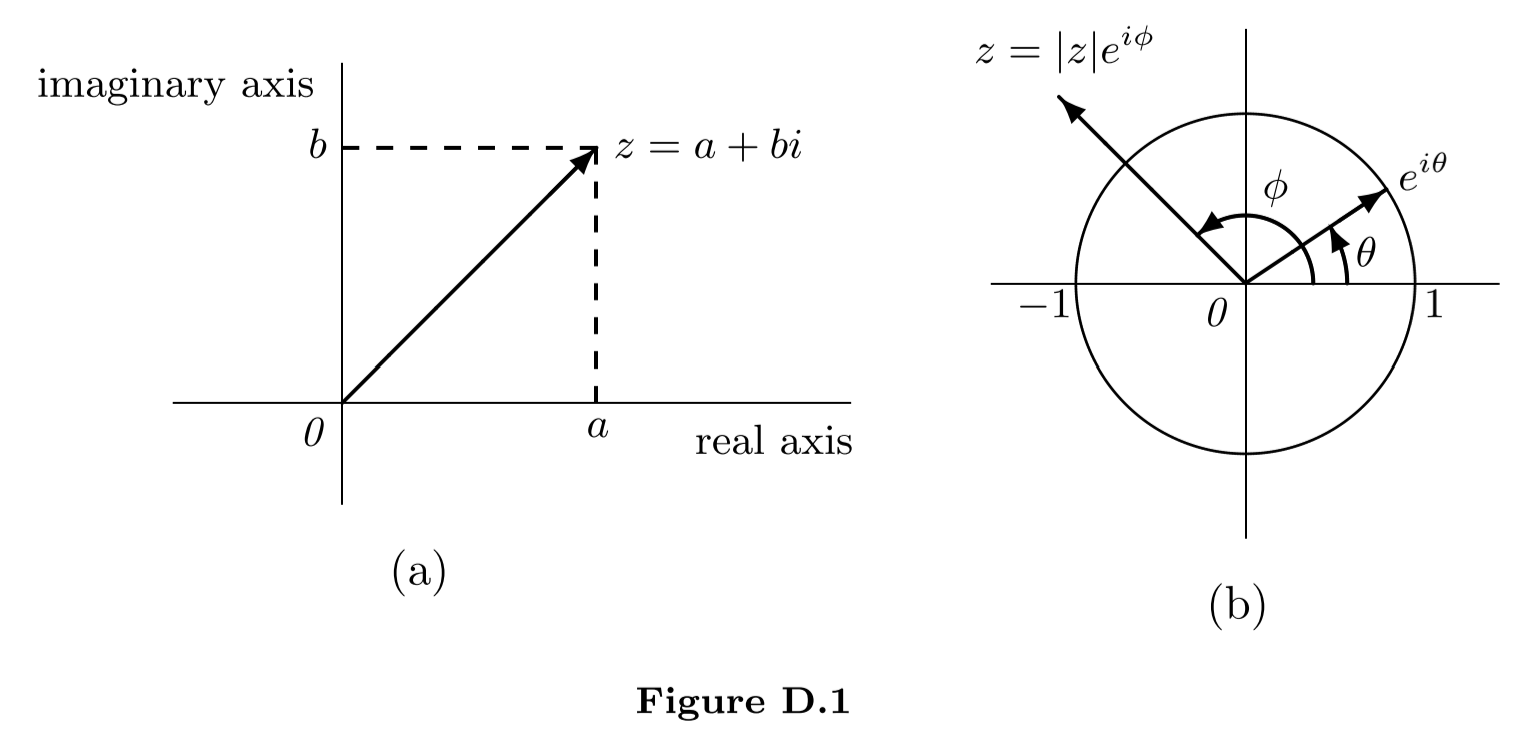
\includegraphics[width=14cm]{images/figure-d-1.png}

\begin{remark} \label{remark d.6}
It is interesting as well as \emph{useful} that complex numbers have both a \emph{geometric and an algebraic representation}.
Suppose that \(z = a + b\iu\), where \(a\) and \(b\) are real numbers.
We may \emph{represent} \(z\) as a vector in the \emph{complex plane} (see Figure D.1(a)).
Notice that, as in \(\SET{R}^2\), there are \emph{two axes}, the \textbf{real axis} and the \textbf{imaginary axis}.
The real and imaginary parts of \(z\) are the first and second coordinates, and the absolute value of \(z\) gives the \emph{length} of the vector \(z\).
It is clear that addition of complex numbers may be represented as in \(\SET{R}^2\) using the parallelogram law.
\end{remark}

\begin{remark} \label{remark d.7}
In \SEC{2.7}, we introduce \href{https://www.wikiwand.com/en/Euler\%27s_formula}{Euler's formula}.
The special case \(e^{\iu \theta} = \cos \theta + \iu \sin \theta\) is of particular interest.
Because of the geometry we have introduced, we may represent the vector \(e^{\iu \theta}\) as in Figure D.l(b);
that is, \(e^{\iu \theta}\) is the \emph{unit vector} that \emph{makes an angle \(\theta\) with the positive real axis}.

From this figure, we see that any \emph{nonzero} complex number \(z\) may be depicted as a multiple of a unit vector, namely, \(z = \abs{z}e^{\iu \phi}\), where \(\phi\) is the angle that the vector \(z\) makes with the positive real axis.
\textbf{Thus multiplication, as well as addition, has a simple geometric interpretation}:
If \(z = \abs{z} e^{\iu \theta}\) and \(w = \abs{w} e^{\iu \omega}\) are two nonzero complex numbers, then from the properties established in
\SEC{2.7} and \THM{d.3}, we have
\begin{align*}
    zw & = \abs{z} e^{\iu \theta} \cdot \abs{w} e^{\iu \omega} & \text{by supposition} \\
       & = \abs{z}\abs{w} e^{\iu \theta} e^{\iu \omega} & \text{of course} \\
       & = \abs{zw} e^{\iu \theta} e^{\iu \omega} & \text{by \THM{d.3}(a)} \\
       & = \abs{zw} e^{\iu (\theta + \omega)} & \text{just exponential algebra for complex numbers, see definition in page 133}
\end{align*}
So \(zw\) is the vector whose length is the product of the lengths of \(zw\), and makes the angle \(\theta + \omega\) with the positive real axis.
\end{remark}

Our \textbf{motivation} for enlarging the set of real numbers to the set of complex numbers is to obtain a field such that
\emph{every polynomial with nonzero degree having coefficients in that field has a zero}.
Our next result guarantees that the field of complex numbers has this property.

\begin{appendix theorem} [The Fundamental Theorem of Algebra] \label{thm d.4}
Suppose that \(p(z) = a_n z^n + a_{n-1} z^{n-1} + ... + a_1 z + a_0\) is a polynomial in \(\mathcal{P}(\SET{C})\) of
degree \(n \ge 1\).
Then \(p(z)\) has a zero.
\end{appendix theorem}

\begin{proof}
Please refer to some analysis course.
\end{proof}

The following important corollary is a consequence of \THM{d.4} and the \emph{division algorithm} for polynomials (\THM{e.1}).

\begin{appendix corollary} \label{corollary d.4.1}
If \(p(z) = a_n z^n + a_{n-1}z^{n - 1} + ... + a_1 z + a_0\) is a polynomial of degree \(n \ge 1\) with \emph{complex} coefficients, then there exist complex numbers \(c_1, c_2, ..., c_n\) (\emph{not} necessarily distinct) such that
\[
    p(z) = a_n(z - c_1)(z - c_2) ... (z - c_n).
\]
\end{appendix corollary}

\begin{proof}
If \(p(z)\) has degree \(1\), then \(p(z) = a_1 z + a_0 = a_1(z + \cfrac{a_0}{a_1})\), which has the desired form.

So assume \(p(z)\) has degree \(n > 1\).
WLOG, we can write \(p(z)\) as
\begin{align*}
    p(z) & = a_n z^n + a_{n-1}Z^{n - 1} + ... + a_1 z + a_0 \\
         & = a_n \left( z^n + \frac{a_{n-1}}{a_n} z^{n - 1} + ... + \frac{a_1}{a_n} z + \frac{a_0}{a_n} \right)
\end{align*}
Now by \THM{d.4}, \(z^n + \cfrac{a_{n-1}}{a_n} z^{n - 1} + ... + \cfrac{a_1}{a_n} z + \cfrac{a_0}{a_n}\) has a zero \(c_1\), so
\[
    z^n + \frac{a_{n-1}}{a_n} z^{n - 1} + ... + \frac{a_1}{a_n} z + \frac{a_0}{a_n} = (z - c_1)q_1(z)
\]
for some \(q_1(z)\) having degree \(n - 1\).
So we have
\[
    p(z) = a_n (z - c_1) q_1(z).
\]
Continue this process \emph{inductively} on \(q_1(z)\), we will get \(p(z) = a_n(z - c_1)(z - c_2) ... (z - c_n)\), as desired.
\end{proof}

\begin{remark} \label{remark d.8}
A field is called \textbf{algebraically closed} if it has the property that every polynomial of positive degree with coefficients from that field factors as a product of polynomials of degree \(1\).
Thus the preceding corollary asserts that the field of complex numbers is algebraically closed.
\end{remark}
